
\chapter{Discussion}
\label{chap8}
This chapter will evaluate how the implemented algorithms work, the shortcomings and
possible solutions to problems. 

\section{How did it perform?}
How the system preformed are outlined in this section. Starting off with the
\emph{SwissRanger 3000} Time-of-Flight camera.

\subsection{MESA SwissRanger 3000}
To start off, the output from the camera were applied directly into matlab. Default
integration time were used, and the intensity- and range images where captured as is from
the camera electronics.

The default readout from the ToF camera were not that affected by the difficulties
described in Chapter \ref{chap2}, but the individual range values where dominated by normal
distributed measurement errors. This where removed by averaging the images over a number
of successive images. This reduced the response time of the sensor and therefor the
refreshment time, but this will most probably not be a case in this application, since the
velocities included are not of the greatest magnitudes. 

Figure \ref{chap8:fig-typical-tof-image} shows a typical range image, and the
corresponding intensity image. 
\begin{figure}[htbp]
    \centering
    %\includegraphics[width=0.8\textwidth]{pics/tof-imagery}
    \caption{Typical range image of the pipe}
    \label{chap8:fig-typical-tof-image}
\end{figure}

When objects came too close to the sensor, it looked like the sensor went berserk. This
was because the intensity values became so large, and they dominated the picture
completely. The solution to this were to filter the range image based on the intensity
value of that pixel. An example of this can be seen in Figure
\ref{chap8:fig-tof-imagery-intensity-filtered}
\begin{figure}[htbp]
    \centering
    %\includegraphics[width=0.45\textwidth]{pics/tof-intensity-unfilterd}
    %\includegraphics[width=0.45\textwdith]{pics/tof-intensity-filtered}
    \caption{The unfiltered and filtered point clouds}
    \label{chap8:fig-tof-imagery-intensity-filtered}
\end{figure}



\subsection{Minoru 3D webcamera}
The stereo camera rig which is used in the project is a cheap mass produced stereo
webcamera. As seen from the calibration in Chapter \ref{chap3} the two different cameras have substantial
distortion, both tangential due to misaligned CCD chip, and radial due to cheap optics.
Unfortunately, the CCD chips are horizontally aligned right, while in the vertical
direction they are aligned in a divergent way. This will limit the field-of-view of the
camera. The principal axes of the two cameras are unaligned horizontally, which will
further limit the field-of-view. See figures \ref{chap2:fig-tang-dist},
\ref{chap3:fig-comp-lensdist} and \ref{chap8:fig-rad-dist}.
\begin{figure}[htbp]
    \centering
    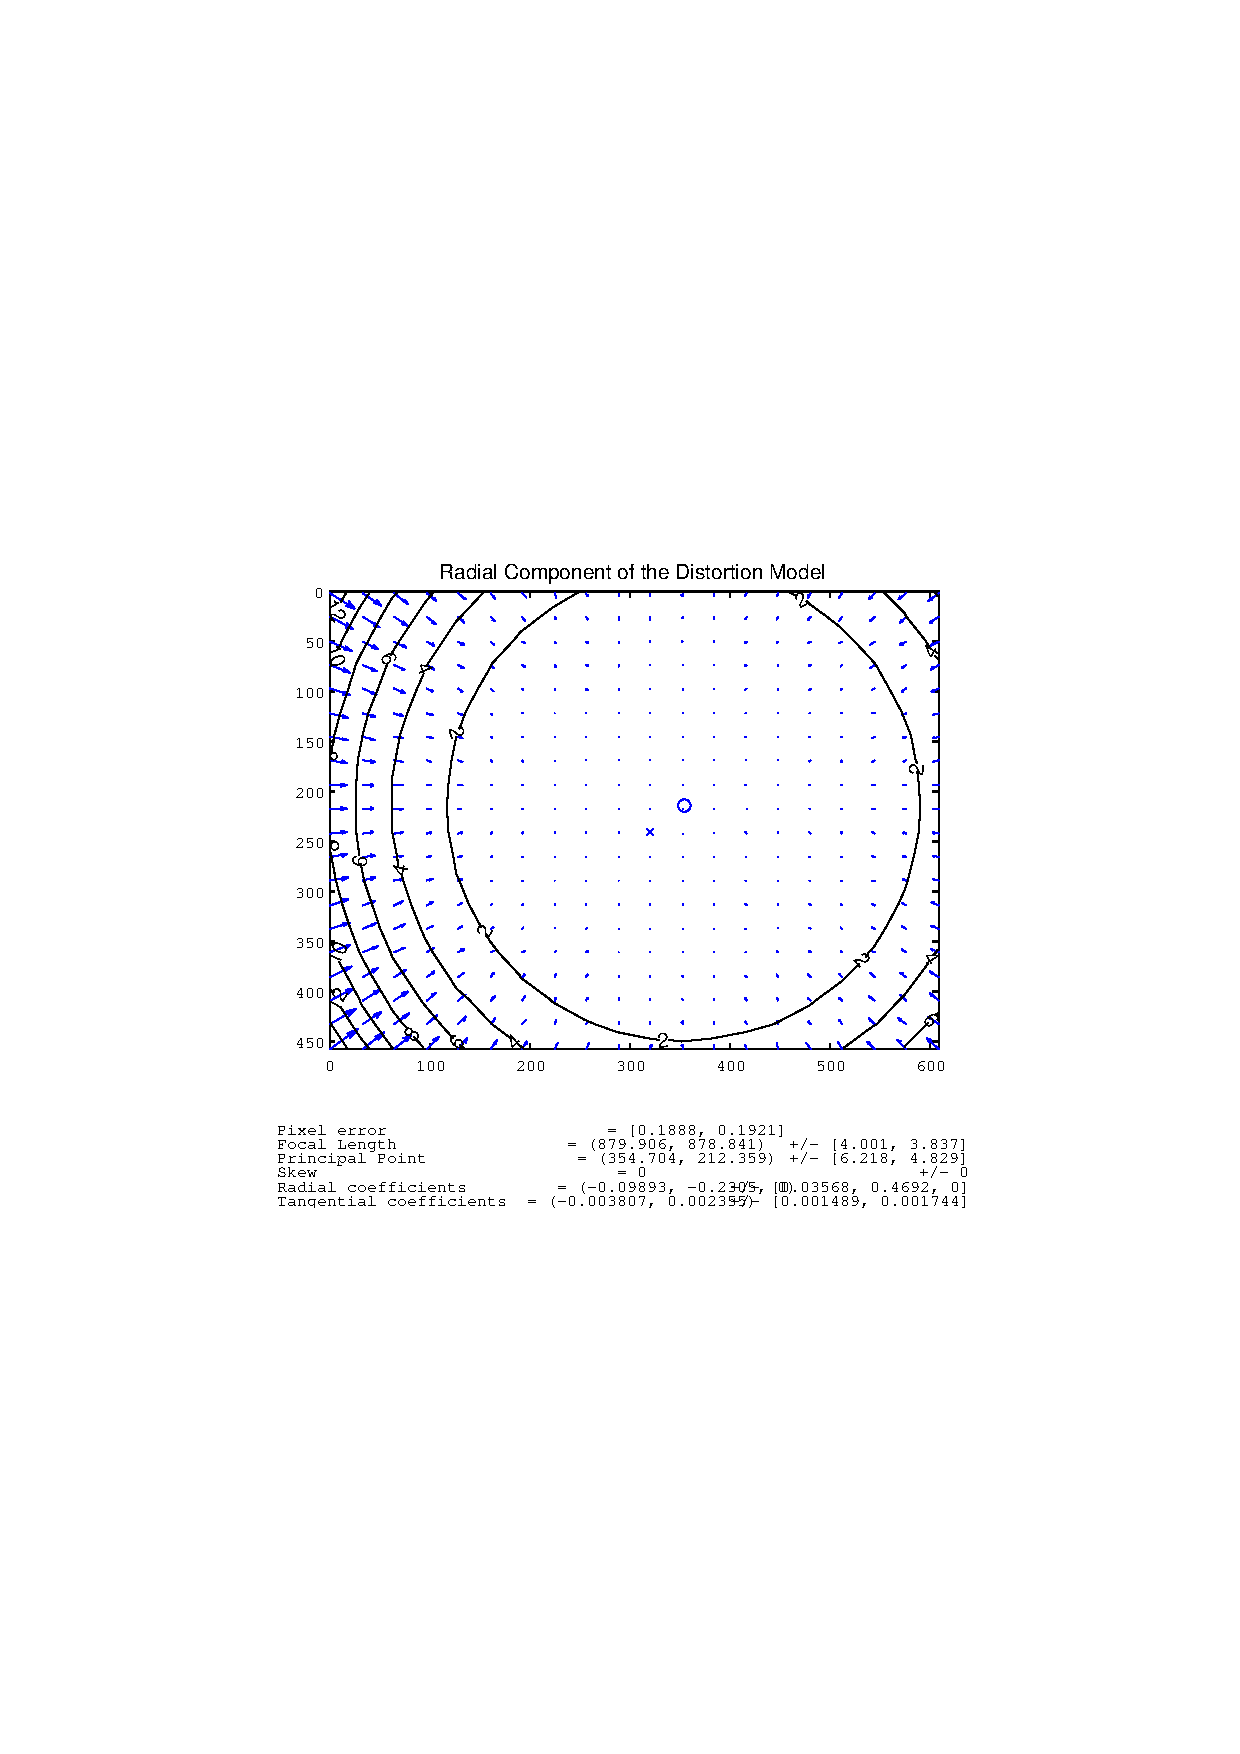
\includegraphics[width=0.45\textwidth]{pics/left_rad_dist}
    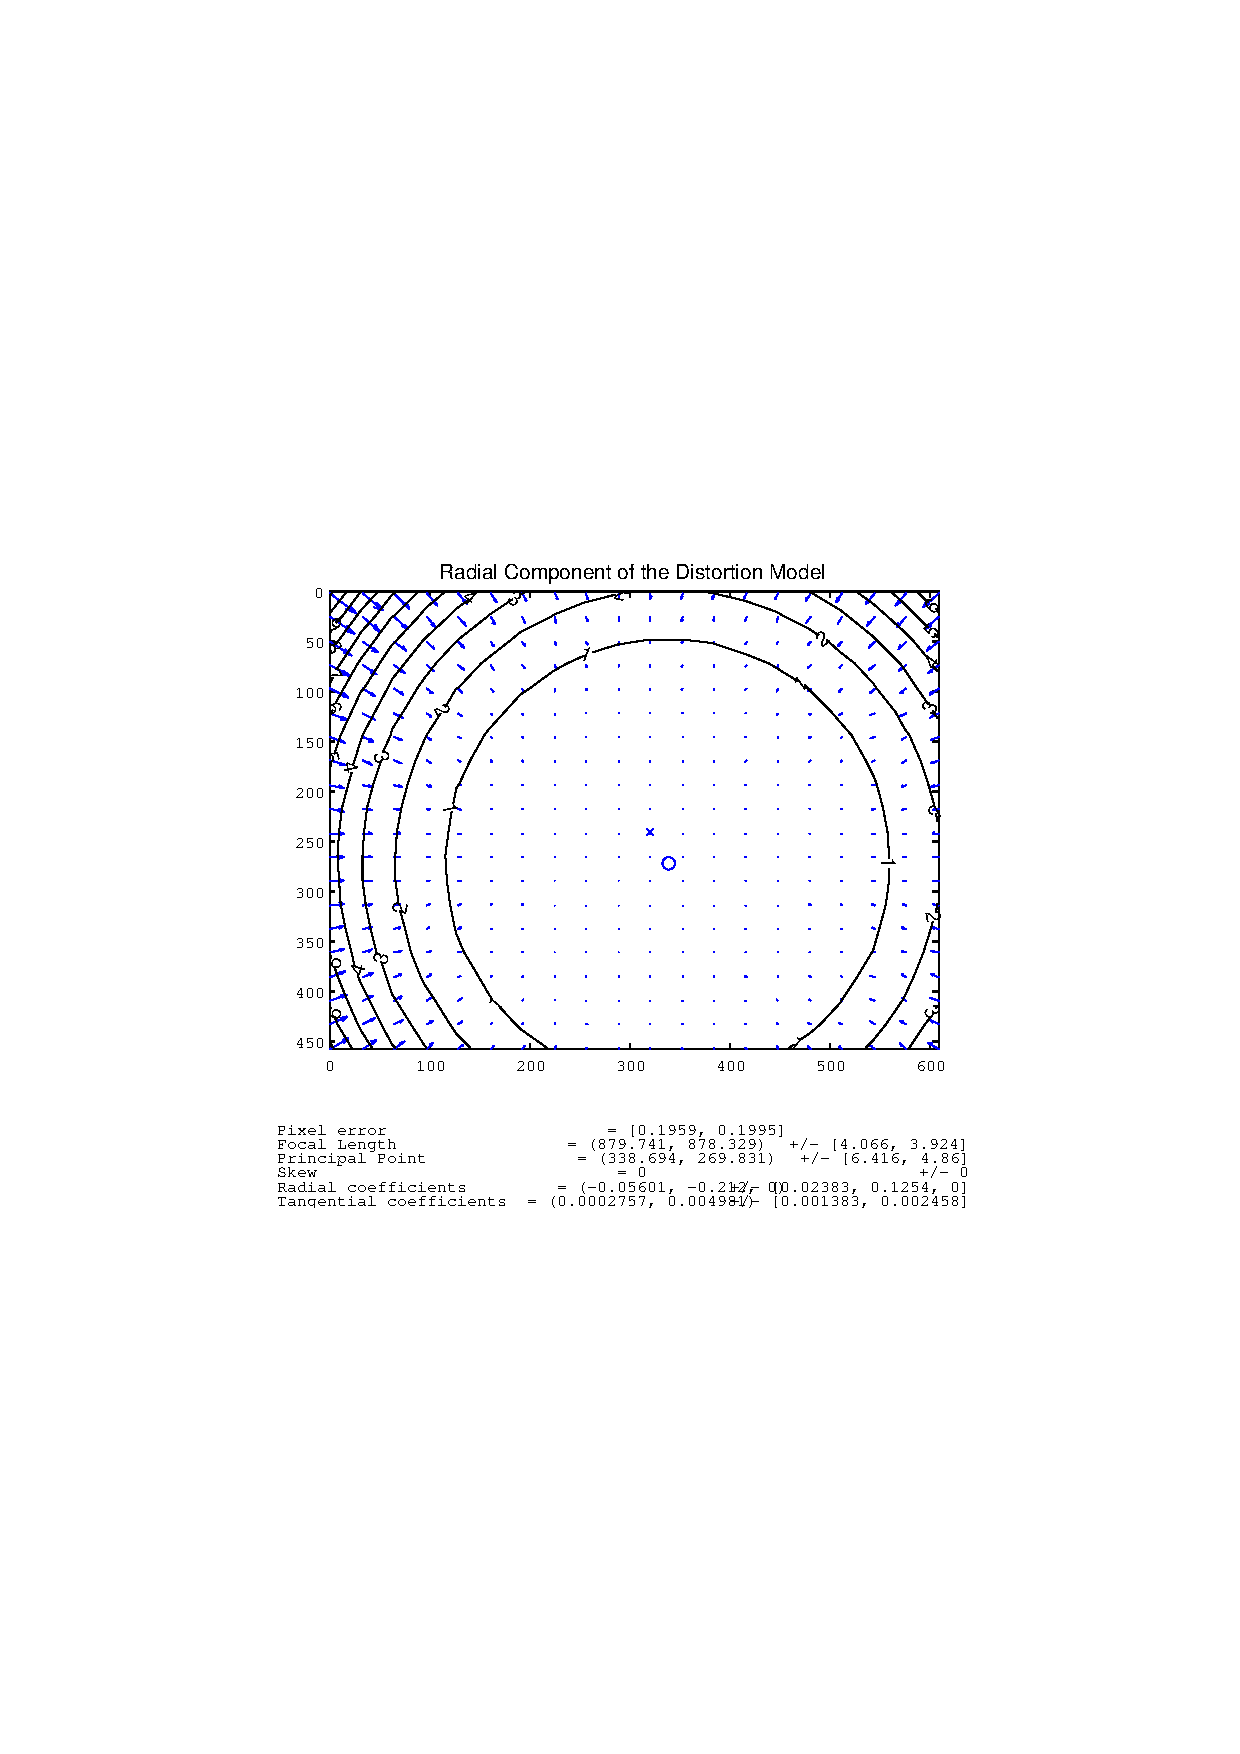
\includegraphics[width=0.45\textwidth]{pics/right_rad_dist}
    \caption{The radial distortions of the left and right camera of the stereo rig}
    \label{chap8:fig-rad-dist}
\end{figure}
The field-of-view of the stereo rig is the incision of the two images. 

Another limit of the cameras, besides the field-of-view is the light sensitivity and
the amount of noise on the captured images. The amount of noise in the captured pictures
are dependant on the portion of ambient light in the scene. In the tests no extra
light source where used, only ambient and sunlight from the surroundings. This was because
the pipe bends where turned towards the window which gave much sunlight. If a artificial
light source were included in the tests, some of the features would be sharper and the
matching would have produced better results. 

The inside of the test pipe were mostly featureless. The implemented algorithms did not
detect enough features in both cameras to calculate a dense stereo image of in most of the
cases. 

Even when there were obstacles, both irregular and regular objects, the algorithm did not
detect enough features, and where not able to match these features. This might be because
that there were not enough light in the scene, and the surfaces of the irregular object
where not sharp enough for the algorithm to detect. 

To test if the algorithm did provide dense stereo images, the stereo rig were directed at
a typical lab environment, with enough structure to make good stereo matches for the
implementation. See figures \ref{chap8:fig-structured-test-rectified} and
\ref{chap8:fig-structured-test-depth}
\begin{figure}[htbp]
    \centering
    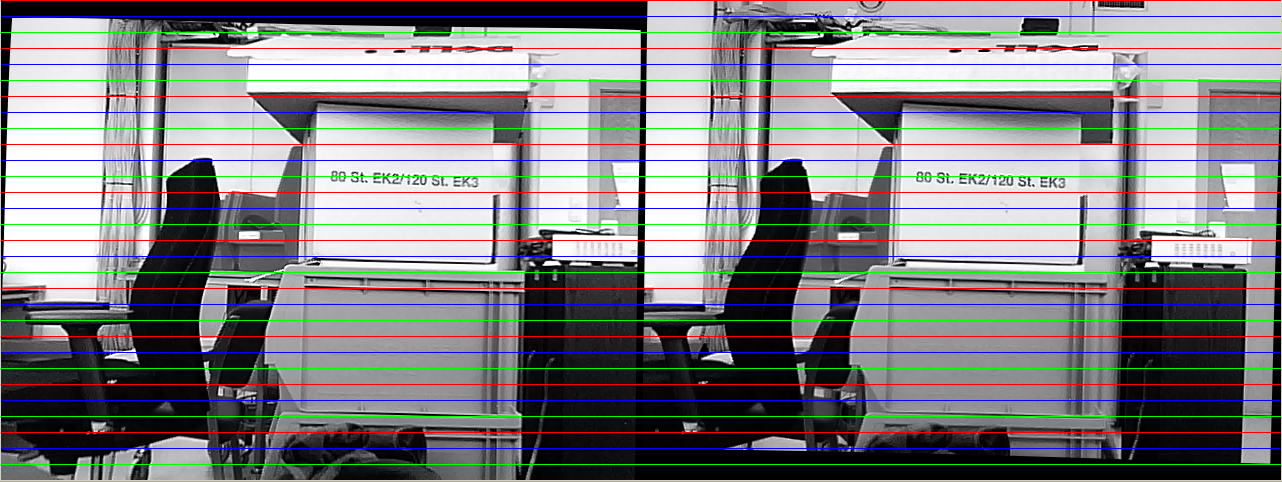
\includegraphics[width=\textwidth]{pics/structure-test-rectified}
    \caption{Rectified left and right images of the structured lab environment}
    \label{chap8:fig-structured-test-rectified}
\end{figure}
The rectified images have horizontal lines superimposed, are to verify that the same
pixels that are in both images are aligned horizontally.
\begin{figure}[htbp]
    \centering
    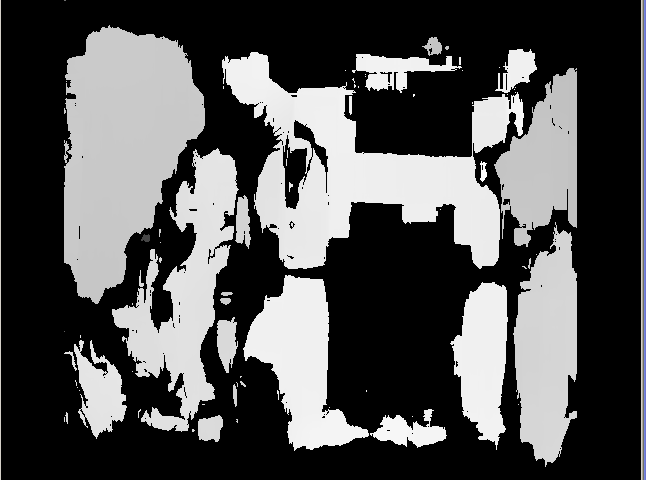
\includegraphics[width=0.45\textwidth]{pics/structure-test-depth}
    %\includegraphics[width=0.45\textwidth]{pics/structured-test-3d}
    \caption{Depth image and projected point cloud of the structured lab environment test}
    \label{chap8:fig-structured-test-depth}
\end{figure}
This clearly shows that the rectification and finding stereo correspondences
works adequately for good lit, structured
environments. The depth image is represented in pixel related units. Since the exact size
of the pixels on the CCD chip were difficult to come by, the distances are given in
pixels. It can be seen that the range image is much more detailed, this is most probably
because there are sufficient light in the scene and a lot more features which can be
matched.

When regarding speed, the \emph{OpenCV} library are reasonable fast. When running at
$640\times480$ a brute-force implementation of the stereo matching using standard
\emph{OpenCV}-library methods, where able to process 2-3 stereo pairs each second, and
output a dense stereo range image, on a Pentium 4 3.0 GHz Windows XP standard workstation
with 2 Gb of RAM. 



\subsection{Hokuyo URG-04LX Laser Range Finder}
The measurement from the laser range finder that affects the readings in the test were
mostly random gaussian distributed noise. To get rid of this, 5 successive
readings where averaged. Since the update rate of the range finder is 10 Hz, the system
will get readings from the URG twice every second. This will not impact the control system
that much, since the dynamics of the system is not that fast. The implementation, the time
needed to get a full range scan was about 0.1-0.15 seconds. The times seemed a bit random,
and where dependant on the time to locate enough memory to store the scan. 



\subsection{Surface Fit and Pipe Properties Estimation}
The proposed surface fit algorithm is based on least-squares. This does not work very good
when there is no segmentation employed in the system. Looking at Figure
\ref{chap7:fig-longpipe-tof-3d} from the Long pipe test, the first cylinder axis is severely displaced. This
is because of pipeline profile. The Y-junction draws is recognized as half a cylinder. The
other cylinders are however fitted better to the point cloud. Although the axis are
directed upwards. The direction vectors are given below in Equation
\eqref{chap8:eq-direction-longpipe}. 
\begin{equation}
    \label{chap8:eq-direction-longpipe}
    a_1 = \left[ \begin{matrix}
                        0.8165\\
                       -0.1749\\
                       0.5503 
                 \end{matrix} \right] \quad a_2 = \left [
                 \begin{matrix}
                       0.0009\\
                       0.08657\\
                       0.9963
                 \end{matrix} \right] \quad a_3 = \left [
                 \begin{matrix}
                       -0.0997\\
                       0.1185\\
                       0.9879
                 \end{matrix} \right]
\end{equation}
Vector $a_2$ and $a_3$ are almost parallel with the z-axis, which is the view direction,
and also the direction of the pipe. But the axis are offset in the y-direction which tilts
the cylinder axis upwards. This is due to the uneven distribution of points in the top of
the pipe, and because of the least-squares approach the axis are drawn towards the largest
clustering of points. 

Figure \ref{chap7:fig-longpipe-tof-dist} is a measure on how good the cylinder fits. The
figure have small crosses where the next next cylinder interval starts. The x-axis show
the number of points which is fitted to the cylinder, and the y-axis scale is in meters.
As seen from the figure, the overall distance of the points to the given cylinders are in
general less than 5 cm, this is not a great result, but it suffices and gives the general
direction of the pipe. This collection of points might be used for a crude selection
criterion for which point indices that might belong to the cylinder. The algorithm might
then be run once more on the filtered point selection, and give a better cylinder fit to
selected set. 

For the Laser Range finder data, on this test, the line fitting worked quite well, see
Figure \ref{chap7:fig-longpipe-urg-2d}. For the horizontal lines, the walls of the pipe
are detected adequately. The error of the for the fitted horizontal lines are oscillating
around zero, except for the ends of the lines. The vertical line fit , which
really is transversal lines in the plane, are another story. The histogram bins for the
vertical lines where chosen large in this test, and this can be seen because all the lines
which really should have been vertical on the figure are either drawn to the left or right
of the vertical axis. 
\begin{figure}[htbp]
    \centering
    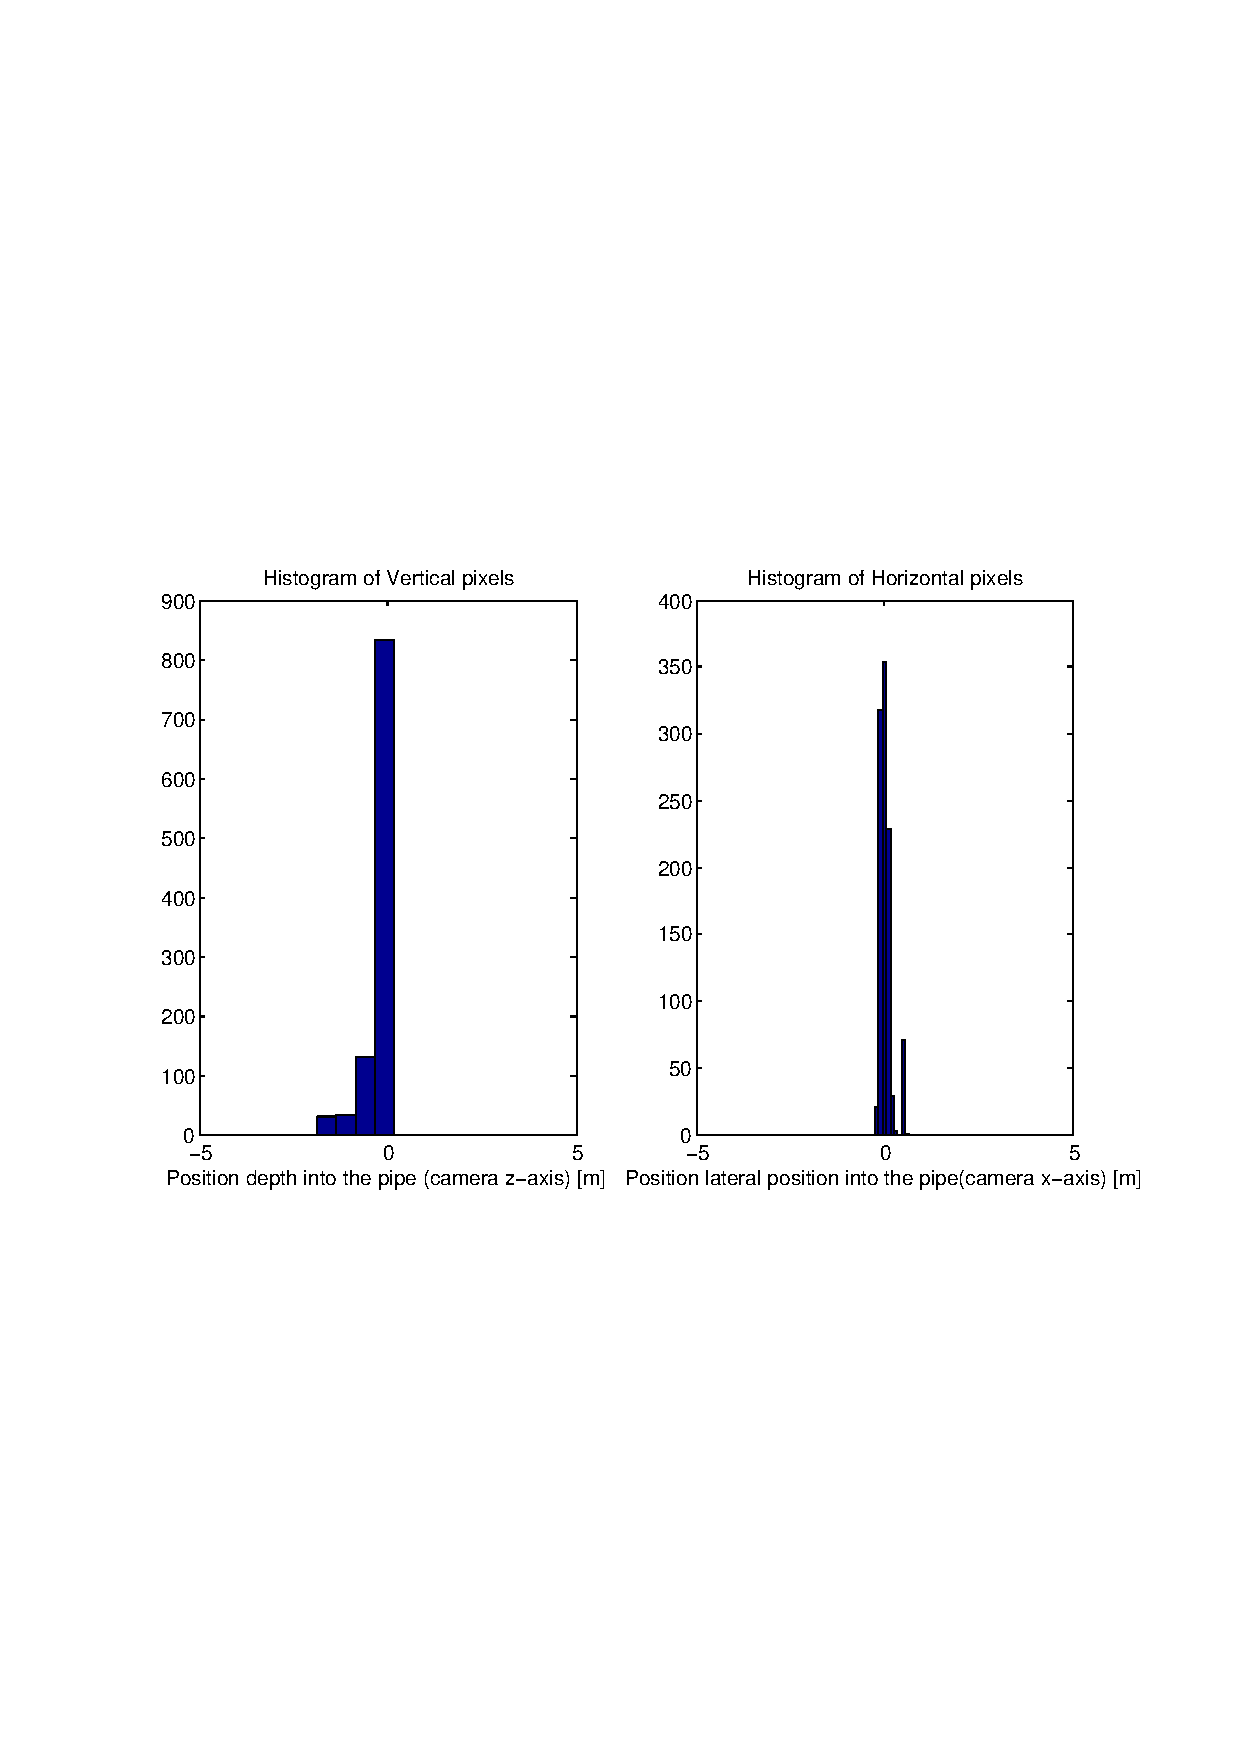
\includegraphics[width=0.8\textwidth]{pics/longpipe-urg-hist}
    \caption{The histogram for the vertical and horizontal line fit for the long pipe test}
    \label{chap8:fig-longpipe-urg-hist}
\end{figure}
Figure \ref{chap8:fig-longpipe-urg-hist} shows the distribution of the points in the
histogram binds. As seen, there are most points in the bin containing the origin, this is
because of the sectors of the laser range finder which cannot be measured. This points are
not removed from the data set, but not included in the line fitting algorithm. 
The second plot in the figure clearly shows that there are three distinct gathering of
points with almost the same y-coordinates, which makes up the three walls of as seen on
Figure \ref{chap7:fig-longpipe-urg-2d}.

\section{Why did it perform this way?}



